\documentclass{beamer}

\usepackage{framed}
\usepackage{subfiles}
\usepackage{graphicx}
\begin{document}
\subfile{02-teaching.tex}
\subfile{01-boxplots.tex}
\subfile{01-histograms.tex}
\subfile{02-statsbase.tex}
\subfile{04-dougbates.tex}
\subfile{04-mixedmodels.tex}
\subfile{04-OnlineStats.tex}
\end{document}
%==============================================%
\begin{frame}
	\frametitle{Statistics with Julia}
	\large
	
	Who am I?
	
	Python vs R vs Julia in the University Class Room
	
	Matlab, SPSS, MINITAB
	
	Technology Acceptance Models
	
	Why is this important?
	
	--------------------------------------------------
	Julia vs Matlab
	
\part{title}


	
	---------------------------------------------------
	What I miss
	Sampling
	Weighted Sampling
	Frequency Tables
	
	--------------------------------------------------
	
	Why use R?
	why use Julia
	
	I (used to) teach Math Science and Computer Science Students
	
	Maths > MatLab
	CompSci > Java
	
	Legacy
	
	
\end{frame}
%==============================================%
\begin{frame}
	\frametitle{Statistics with Julia}
	\large
	
%	Automate all the things
\begin{figure}
\centering

\includegraphics[width=0.95\linewidth]{images/AutomateAllTheThings}

\end{figure}
	
\end{frame}

%==============================================%

\section{Teaching Undergrads}



%
%sampling - sample
%
%summarystats - can you make a trimean?
%
%Gambler's Ruin Graphic of Distribution
%
%HypothesisTesting.jl




%========================================================%
\begin{frame}
Types

R is weakly typed
with Julia you have to very particular.

%=========================================================%

Berlin R USER GROUP

Mixed Models


%==========================================================%
\end{frame}

\begin{frame}
	\begin{figure}
\centering
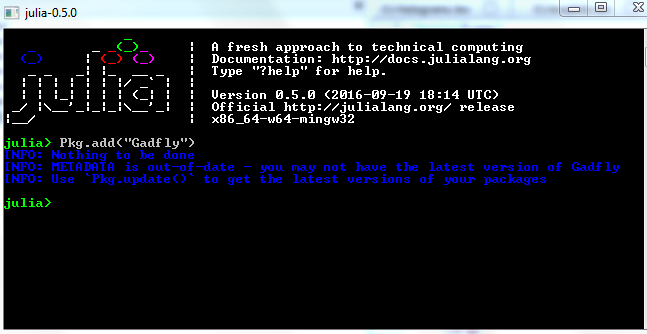
\includegraphics[width=1.05\linewidth]{images/InstallGadfly}
\end{figure}

\end{frame}

\section{Non Parametric Tests}
\begin{frame}
	\frametitle{Non Parametric Tests}
	Nonparametric tests are often used in place of their parametric counterparts when certain assumptions about the underlying population are questionable. For example, when comparing two independent samples, the Wilcoxon Mann-Whitney test does not assume that the difference between the samples is normally distributed whereas its parametric counterpart, the two sample t-test does. Nonparametric tests may be, and often are, more powerful in detecting population differences when certain assumptions are not satisfied.
	
	All tests involving ranked data, i.e. data that can be put in order, are nonparametric.
	
	
\end{frame}


\end{document}
